Диффузионные модели за последние годы стали стандартом для генерации и редактирования изображений по текстовому описанию. Современные архитектуры способны синтезировать фотореалистичные сцены, точно передавать стиль, освещение и текстуры, а также поддерживать разнообразные режимы управления — от inpainting \cite{mao2025unifyedit} до image-to-image \cite{blackforestlabs2025fluxkontext} трансформаций. В типичных сценариях, когда текстовый запрос описывает распространённые объекты и привычные композиции, качество генерации оказывается очень высоким.

Однако у этих моделей есть принципиальное ограничение: многие промпты оказываются для них семантически сложными. Это особенно заметно в случаях, когда текст содержит нетипичные для обучающего распределения концепты или их сочетания, редкие геометрические конфигурации, а также количественные требования. Например, композиционные конструкции («медведь делает стойку на передних лапах в парке»), структурные деформации объектов («гриб в лесу со сломанной пополам ножкой») или количественные требования («перчатка с шестью пальцами»). В подобных случаях модель часто генерирует визуально правдоподобную, но семантически некорректную сцену: игнорирует часть условий, «исправляет» нетипичную деталь на более вероятную либо создаёт гибридную интерпретацию запроса. Такие описания и соответствующие примеры генераций приведены на \autoref{fig:weird_prompts}.

С практической точки зрения эта проблема актуальна. В задачах генерации плохое понимание моделью семантики промпта часто приводит к неправильной генерации. В задачах редактирования, помимо этой проблемы, возникают и другие, например понимание моделью относительного расположения объектов на изображении. Таким образом, повышение семантической точности является краеугольным условием надёжного применения диффузионных моделей как инструмента контролируемого текстом редактирования и генерации изображений.

Корень описанной проблемы заключается в том, что диффузионные модели аппроксимируют распределение обучающих данных. Даже при условной генерации по тексту они склонны стремиться к наиболее привычным визуальным конфигурациям. Когда запрос требует выхода за пределы выученного распределения, например необычных количеств, нетривиальных пространственных отношений или логически противоречивых комбинаций, модель зачастую оказывается неспособна корректно удовлетворить этим требованиям.

\newpage

\begin{figure}[ht]
\centering

\begin{minipage}[t]{0.3\textwidth}
\centering
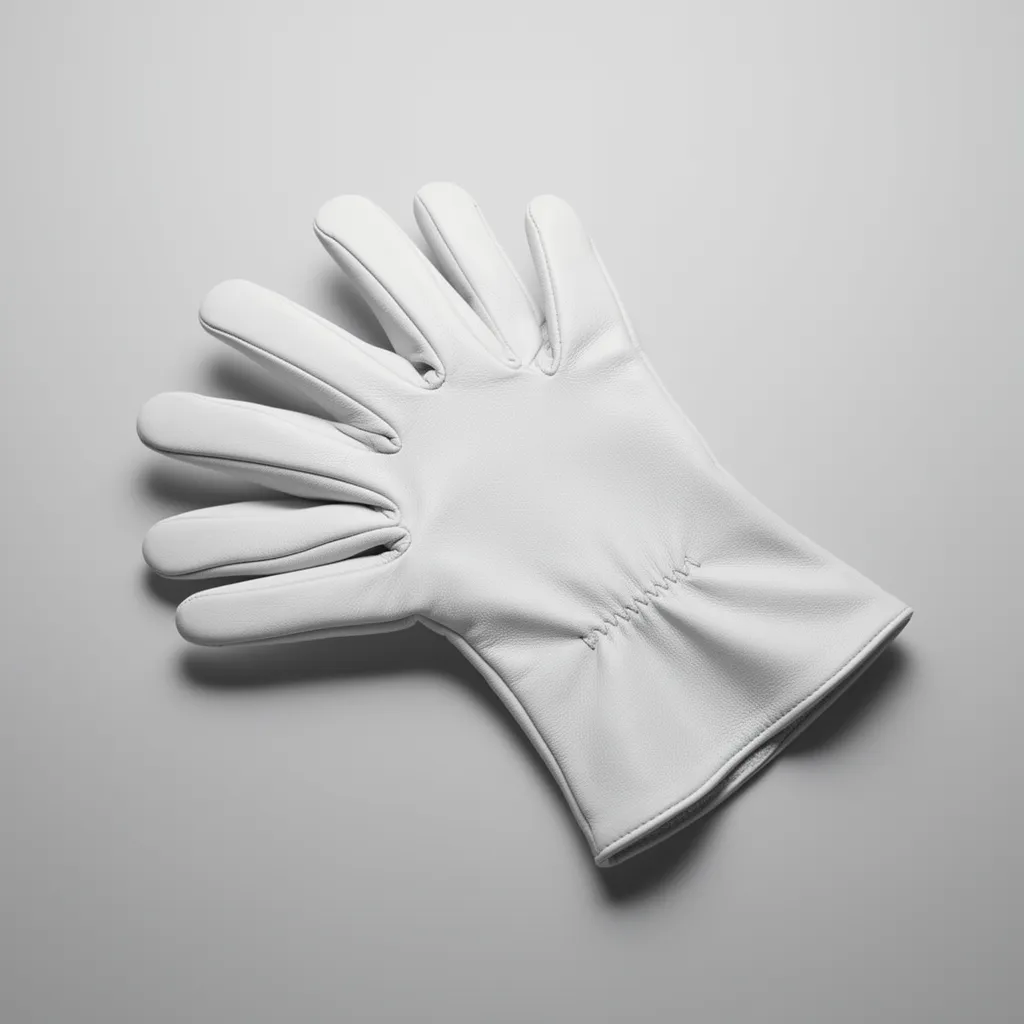
\includegraphics[width=\textwidth]{glove.png}

\small Промпт: «Белая перчатка с шестью пальцами»


\end{minipage}
\hfill
\begin{minipage}[t]{0.3\textwidth}
\centering
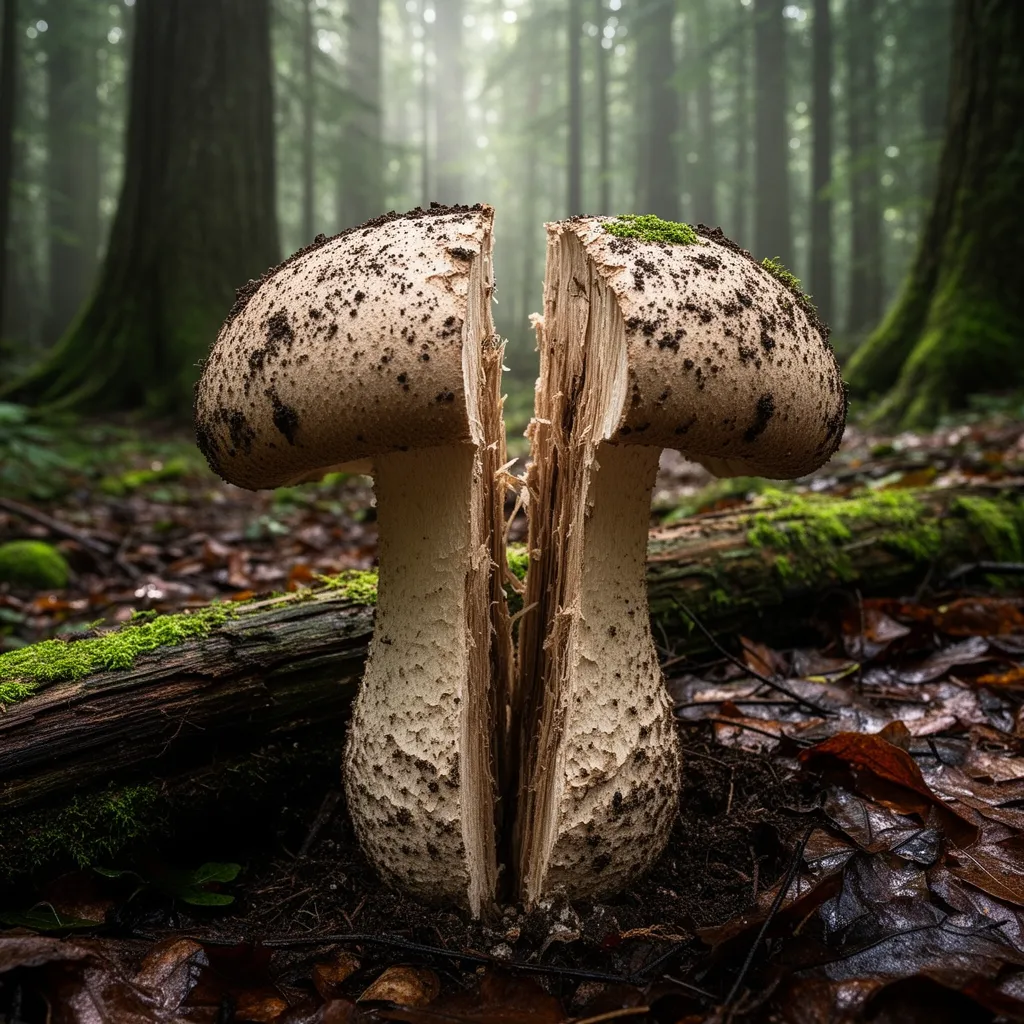
\includegraphics[width=\textwidth]{mushroom.png}

\small Промпт: «Гриб со сломанной пополам ножкой в лесу»


\end{minipage}
\hfill
\begin{minipage}[t]{0.3\textwidth}
\centering
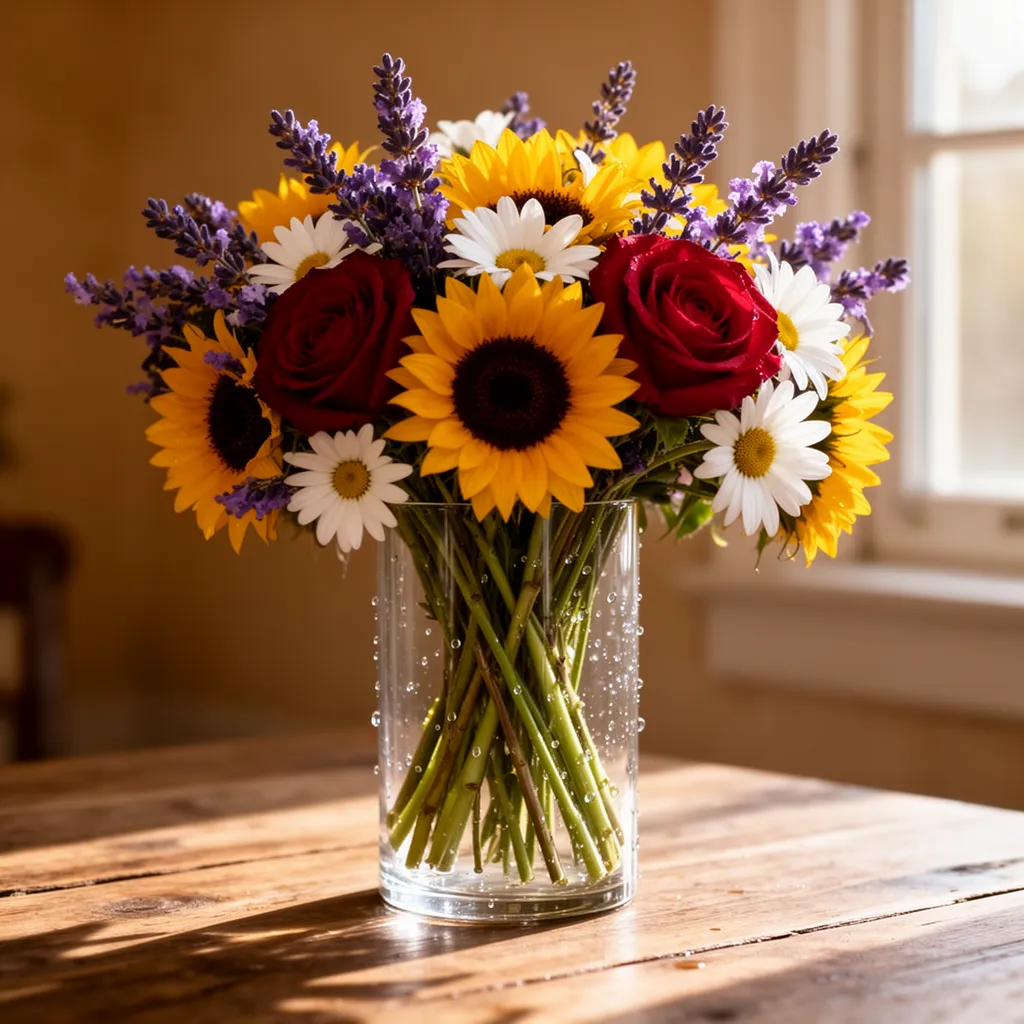
\includegraphics[width=\textwidth]{vase.png}

\small Промпт: «Букет цветов стоит в вазе вверх ногами»


\end{minipage}

\caption{Примеры генерации модели на семантически сложных промптах. Во всех случаях видно, как модель правдоподобно генерирует не соответствующие промпту изображения. Все генерации произведены по переведённым на английский язык промптам моделью FLUX.2[dev].}
\label{fig:weird_prompts}
\end{figure}

В то же время большие vision-language модели (VLM), обученные в авторегрессионной постановке, демонстрируют значительно более сильные способности к семантическому пониманию и проверке согласованности текста и изображения. Они способны понимать сложные языковые конструкции, учитывать контекст и выявлять несоответствия между визуальными и текстовыми данными. Это открывает возможность использовать VLM не только как инструмент оценки, но и как источник градиентного сигнала для управления процессом генерации.

Идея VLM guidance заключается в том, чтобы оптимизировать параметры генерации диффузионной модели по градиенту функции согласованности, вычисляемой VLM. В работе \cite{miao2024noisediffusion} было показано, что оптимизация стартового латентного представления может существенно повысить семантическую точность генерации сложных сцен. В данной работе эта идея развивается дальше: предлагается исследовать оптимизацию не только стартового латента, но и промежуточных латентных состояний в процессе денойзинга, а также других непрерывных параметров генерации. Такой подход потенциально позволяет воздействовать на семантику изображения не однократно в начале процесса, а последовательно корректировать её на протяжении всей траектории генерации.

Цель работы — экспериментально проверить гипотезу о том, что градиенты авторегрессионных VLM могут служить эффективным инструментом управления генерацией и редактированием изображений в случаях сложных, композиционных и количественных семантик. Для этого будет реализован пайплайн VLM-guided оптимизации и проведено сравнение с современными базовыми моделями по метрикам семантического соответствия (CLIP Score и alignment-оценкам на основе VLM) на наборах промптов различной сложности.

Ожидается, что предложенный подход позволит увеличить показатели семантической точности по сравнению с базовыми диффузионными моделями и, в частности, повысить устойчивость генерации в случаях, подобных приведённым на \autoref{fig:weird_prompts}. Кроме того, особое внимание будет уделено применимости метода к задаче редактирования изображений, где требования к сохранению исходного содержания и встраиванию в него корректировок делают проблему ещё более выраженной.

В дальнейшем работа организована следующим образом. В следующем разделе представлен обзор литературы по методам guidance и VLM-based управлению генерацией. Затем формулируется постановка задачи и описываются особенности рассматриваемых моделей и подходов guidance. После этого приводится описание предлагаемого пайплайна и экспериментального протокола. В заключении обсуждаются ограничения подхода и направления дальнейших исследований.